\documentclass[UTF8,a4paper,10pt]{ctexart}
\usepackage[left=2.50cm, right=2.50cm, top=2.50cm, bottom=2.50cm]{geometry}
%页边距
\CTEXsetup[format={\Large\bfseries}]{section} %设置章标题居左

%%%%%%%%%%%%%%%%%%%%%%%
% -- text font --
% compile using Xelatex
%%%%%%%%%%%%%%%%%%%%%%%
% -- 中文字体 --
%\setmainfont{Microsoft YaHei}  % 微软雅黑
%\setmainfont{YouYuan}  % 幼圆    
%\setmainfont{NSimSun}  % 新宋体
%\setmainfont{KaiTi}    % 楷体
%\setmainfont{SimSun}   % 宋体
%\setmainfont{SimHei}   % 黑体
% -- 英文字体 --
%\usepackage{times}
%\usepackage{mathpazo}
%\usepackage{fourier}
%\usepackage{charter}

%\usepackage{helvet}

\usepackage{amsmath, amsfonts, amssymb} % math equations, symbols
\usepackage[english]{babel}
\usepackage{color}	% color content
\usepackage{graphicx}	% import figures
\usepackage{url}	% hyperlinks
\usepackage{bm} 	% bold type for equations
\usepackage{multirow}
\usepackage{booktabs}
\usepackage{epstopdf}
\usepackage{epsfig}
\usepackage{algorithm}
\usepackage{algorithmic}
\usepackage{listings}
\usepackage{xcolor}
\usepackage{booktabs}
\usepackage{zhnumber}
\usepackage{longtable}
\usepackage{subfigure}
\usepackage{float}
\usepackage{caption}
\usepackage{subfigure}
\renewcommand\thesection{\zhnum{section}}
\renewcommand \thesubsection {\arabic{section}}
\renewcommand{\algorithmicrequire}{ \textbf{Input:}}
% use Input in the format of Algorithm  
\renewcommand{\algorithmicensure}{ \textbf{Initialize:}}
% use Initialize in the format of Algorithm  
\renewcommand{\algorithmicreturn}{ \textbf{Output:}}
% use Output in the format of Algorithm  
%%%%%%%%%%%%%%%%%%
\usepackage{listings}
\usepackage{color}
\definecolor{dkgreen}{rgb}{0,0.6,0}
\definecolor{gray}{rgb}{0.5,0.5,0.5}
\definecolor{mauve}{rgb}{0.58,0,0.82}
\lstset{frame=tb,
  language=Python,
  aboveskip=3mm,
  belowskip=3mm,
  showstringspaces=false,
  columns=flexible,
  basicstyle={\small\ttfamily},
  numbers=left,%设置行号位置none不显示行号
  %numberstyle=\tiny\courier, %设置行号大小
  numberstyle=\tiny\color{gray},
  keywordstyle=\color{blue},
  commentstyle=\color{dkgreen},
  stringstyle=\color{mauve},
  breaklines=true,
  breakatwhitespace=true,
  escapeinside=``,%逃逸字符(1左面的键),用于显示中文例如在代码中`中文...`
  tabsize=4,
  extendedchars=false %解决代码跨页时,章节标题,页眉等汉字不显示的问题
}

%%%%%%%%%%%%%%%%%%%%%%%%%%%%
\usepackage{fancyhdr} %设置页眉、页脚
\pagestyle{fancy}
\lhead{}
\chead{}
%\rhead{\includegraphics[width=1.2cm]{fig/ZJU_BLUE.eps}}
\lfoot{}
\cfoot{}
\rfoot{}
\fancyfoot[RE,RO]{~\thepage~}

\fancyhead[RE,RO]{计算物理导论 \quad 2022春季学期 \quad 作业8  \quad 何翼成}

%%%%%%%%%%%%%%%%%%%%%%%
%  设置水印
%%%%%%%%%%%%%%%%%%%%%%%
%\usepackage{draftwatermark}         % 所有页加水印
%\usepackage[firstpage]{draftwatermark} % 只有第一页加水印
% \SetWatermarkText{Water-Mark}           % 设置水印内容
% \SetWatermarkText{\includegraphics{fig/ZJDX-WaterMark.eps}}         % 设置水印logo
% \SetWatermarkLightness{0.9}             % 设置水印透明度 0-1
% \SetWatermarkScale{1}                   % 设置水印大小 0-1    

\usepackage{hyperref} %bookmarks
\hypersetup{colorlinks, bookmarks, unicode} %unicode

\title{\textbf{TSSP方法求解一维G-P方程}}
\author{ 何翼成 \thanks{学号:520072910043; \newline
    邮箱地址:heyicheng@sjtu. edu. cn} }
\date{\today}

\begin{document}
\maketitle

%\begin{abstract}
%这是一篇中文小论文。这个部分用来写摘要。摘要的章标题默认是英文,还没找到改成中文的方法:(
%\end{abstract}
\section*{Project 1}
\section{题目分析}
%%%以下为插入图片模板
%\quad \newline
	\begin{figure}[!htbp]
		\centering
		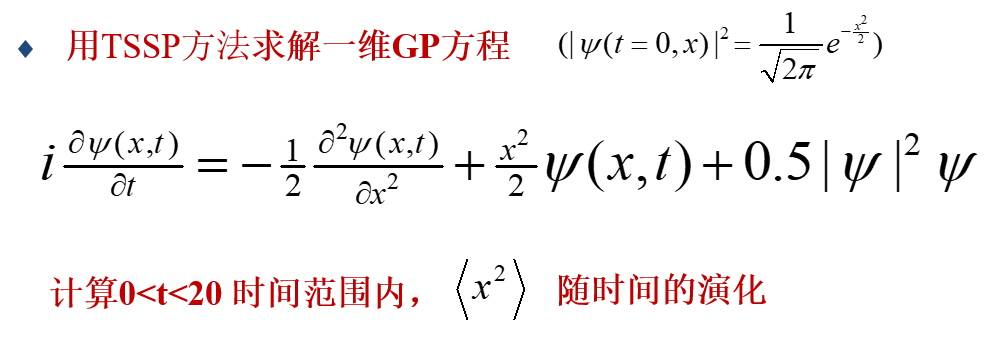
\includegraphics[width=1\textwidth,height=0.2\textwidth]{pictures/pro.png}
		\caption{题目总览} \label{project1}
	\end{figure}

  本题的思路是利用Strang-Splitting Method对该方程进行时间算子分裂法的求解,其中还要还要用到对一阶时间偏微分的近似进行求解。


\section{代码展示}
\lstset{language=matlab}
\begin{lstlisting}
  clear;clc;
  a=-39;b=39;%求解范围
  dx=0.1;%空间格点距离
  M=(b-a)/dx;
  x=a:dx:b;
  phi20=1/sqrt(2*pi)*exp(-x.^2/2);%粒子初态
  phi0=sqrt(phi20);
  dt=0.1;
  t=0:dt:20;%时间
  tlength=length(t);
  eps=1;%eps表示epsilon
  phi_series=zeros(tlength,M+1);%存储phi(x,t)
  phi_xx=zeros(1,M+1);%临时存储
  phi_series(1,:)=phi0;
  l=-M/2:1:M/2-1;
  miu_l=2*pi*l/(b-a);%提前编号
  phi_l=zeros(1,length(l));
  phi_star2=zeros(1,length(x));
  x2=zeros(1,tlength);
  
  for nn=1:tlength-1
  %处理第一部分
      %更新数据
      phi=phi_series(nn,:);
      phi2=phi.^2;
      %phi_pub=[0,phi,0];
  %离散法求解二阶空间导数phi_xx
      %for num=1:M+1
          %phi_xx(num)=(phi_pub(num)+phi_pub(num+2)-2*phi_pub(num+1))/(dx)^2;
      %end
      %phi=phi+1i*eps/2*phi_xx*dt;
      %试用新方法
      phi=phi+1i*dt^3/2*phi;
  %处理第二部分  
      phi_star=exp(-1i*(x.^2/2+0.5*phi2)*dt/(2*eps)).*phi;
  %phi_l是phi_star的傅里叶系数
      for ll=1:length(miu_l)
          phi_l(ll)=sum(phi_star.*exp(-1i*miu_l(ll)*(x-a)));
      end
  %phi**的计算
      for num=1:length(x)
          phi_star2(num)=1/M*sum(exp(-1i*eps*dt.*miu_l.^2/2).*phi_l.*exp(1i*miu_l.*(x(num)-a)));
      end
  %phi(n+1/2)的计算
      phi=exp(-1i*(x.^2/2+0.5*abs(phi_star2).^2)*dt/(2*eps)).*phi_star2;
  %phi(n+1)的计算
      %phi_pub=[0,phi,0];
      %for num=1:M+1
       %   phi_xx(num)=(phi_pub(num)+phi_pub(num+2)-2*phi_pub(num+1))/(dx)^2;
      %end
      %phi=phi+1i*eps/2*phi_xx*dt;
      phi=phi+1i*dt^3/2*phi;
      %每一轮计算都进行归一化
      co=1/sqrt(sum(abs(phi).^2)*dx);
      phi_series(nn+1,:)=co*phi;%每一轮计算都进行归一化
      clc;
      disp("已完成第"+nn+"轮计算,总共有"+tlength+"轮,目前进度"+nn/tlength*100+"%")
  %计算<x^2>的期望值
      x2(nn)=sum(abs(phi_series(nn,:)).^2.*x.^2*dx)/(sum(abs(phi_series(nn,:)).^2*dx));
      if nn==tlength-1
          nn=nn+1;
          x2(nn)=sum(abs(phi_series(nn,:)).^2.*x.^2*dx)/(sum(abs(phi_series(nn,:)).^2*dx));
          disp("已完成第"+nn+"轮计算,总共有"+tlength+"轮,目前进度"+nn/tlength*100+"%")
      end
  end
  plot(t,x2,'k')
  xlabel('Time')
  ylabel('<x^2>')
\end{lstlisting}

\section{结果分析与结论}


	\begin{figure}[!htbp]
		\centering
		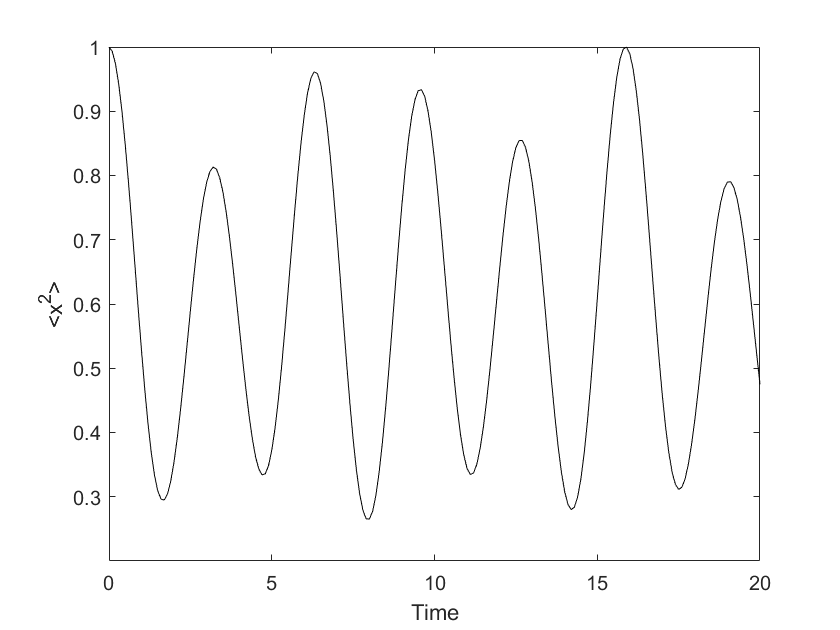
\includegraphics[width=0.5\textwidth,height=0.4\textwidth]{pictures/x22.png}
		\caption{<x^2>在t\in [0,20]的演化情况} \label{p1}
	\end{figure}
由此可以得到$<x^2>$在$t\in[0,20]$的演化情况。


  %%%%%%%%%%%%%%%%%%%%%%%%%第二题%%%%%%%%%%%%%%%%%%%%%%%%%%%%%%%%%
  %%%%%%%%%%%%%%%%%%%%%%%%%第二题%%%%%%%%%%%%%%%%%%%%%%%%%%%%%%%%%
  %%%%%%%%%%%%%%%%%%%%%%%%%第二题%%%%%%%%%%%%%%%%%%%%%%%%%%%%%%%%%
  %%%%%%%%%%%%%%%%%%%%%%%%%第二题%%%%%%%%%%%%%%%%%%%%%%%%%%%%%%%%%
\
%以下为插入代码模板
%~\\
%\lstset{language=matlab}
%\begin{lstlisting}
%\end{lstlisting}


%%%以下为插入图片模板
%\quad \newline
%	\begin{figure}[!htbp]
%		\centering
%		\includegraphics[width=0.5\textwidth,height=0.375\textwidth]{pictures/minscale.png}
%		\caption{最小风向} \label{minsacle}
%	\end{figure}

%%%以下为插入图片模板
%\quad \newline
%	\begin{figure}[!htbp]
%		\centering
%		\includegraphics[width=0.5\textwidth,height=0.375\textwidth]{pictures/minscale.png}
%		\caption{最小风向} \label{minsacle}
%	\end{figure}

%    \begin{algorithm}
%		\caption{Title of the Algorithm}
%     	\begin{algorithmic}[1]
%			\REQUIRE some words.  % this command shows "Input"
%			\ENSURE ~\\           % this command shows "Initialized"
%			some text goes here ... \\
%			\WHILE {\emph{not converged}}
%			\STATE ... \\  % line number at left side
%			\ENDWHILE
%			\RETURN this is the lat part.  % this command shows "Output"
%		\end{algorithmic}
%	\end{algorithm}

\end{document}